%# -*- coding: utf-8-unix -*-
%%==================================================
%% chapter_2.tex for SJTU Master Thesis
%%==================================================

\chapter{时间序列样本统计方法}
\label{chap:1588_theory}
在本章中,将依据对IEEE1588时钟同步原理及协议中可能存在的一些应用问题进行分析,并梳理关于这些问题的当今研究理论成果来作一个全面的分析。

\section{IEEE1588时钟同步原理}
IEEE1588系统是由PTP设备和非PTP设备结合而成的分布式网络化系统。IEEE1588协议主要介绍的是系统中的实时PTP设备之间的相互同步方案,使得所有的从时钟能够与自己的主时钟同步,而所有主时钟又能够和同一个Grand Master时钟同步,最终达到整个系统中所有时钟保持同步。

首先,每个PTP时钟会有多个端口,当系统启动时,会立即开始PTP网络建立过程。该过程中,每个端口会对外发送Announce报文,同时通过检查所收到的Announce报文中的相关信息来判定哪个端口适合成为主时钟,被判定为主时钟的端口则会定期对外发送Sync报文。如果,一个判定为主时钟的端口收到了一个来自于更好的主时钟的Sync报文,那么该主时钟则会立即将自身的主时钟状态切换为从时钟状态。当然,如果一个处于从时钟状态的端口认为自己比当前主时钟更加好,那么它可以将自己设置为主时钟状态,并对外发送Sync报文。当所有端口通过互相比较时钟特性并建立了各自的主从状态后,则意味着主从秩序完成建立。如果此时新加入了一个时钟,那么该时钟首先会等待来自某一主时钟的Sync报文,若在规定的时间内没有收到任何主时钟的Sync报文,那么该时钟则将自身设置为主时钟,直到发现一个更好的主时钟。

随后,则会进行时钟同步过程。该过程主要是主从时钟之间发送报文,使得每个从时钟计算出自身与主时钟之间的时钟偏差,并且对自身进行校正从而实现同步。首先主时钟会对外界进行周期性的Sync报文发送,对于采用硬件时间戳的设备将直接在Sync报文内记录发送时间,否则的话将再发送Follow\_up报文来进行发送。当从时钟收到Sync报文后,则能够接受到发送时间戳并记录当前的接收时间戳。同时,从时钟自身也会周期性向主时钟发送Delay\_Req报文,会通过接受主时钟回传的Delay\_Resp报文来共同计算出链路延时$T_{delay}$和主从偏差$T_{offset}$。最终利用$T_{offset}$对从时钟进行校正而实现同步。
\label{sec:1588_theory_sync}
在图\ref{fig:process_of_time_sync}中,可以看到较为完整的时钟同步过程。下面,对时钟同步过程及相关计算做简明扼要地介绍。

\begin{figure}[htbp]
  \centering
  \begin{minipage}[b]{0.6\textwidth}
    \captionstyle{\centering}
    \centering
    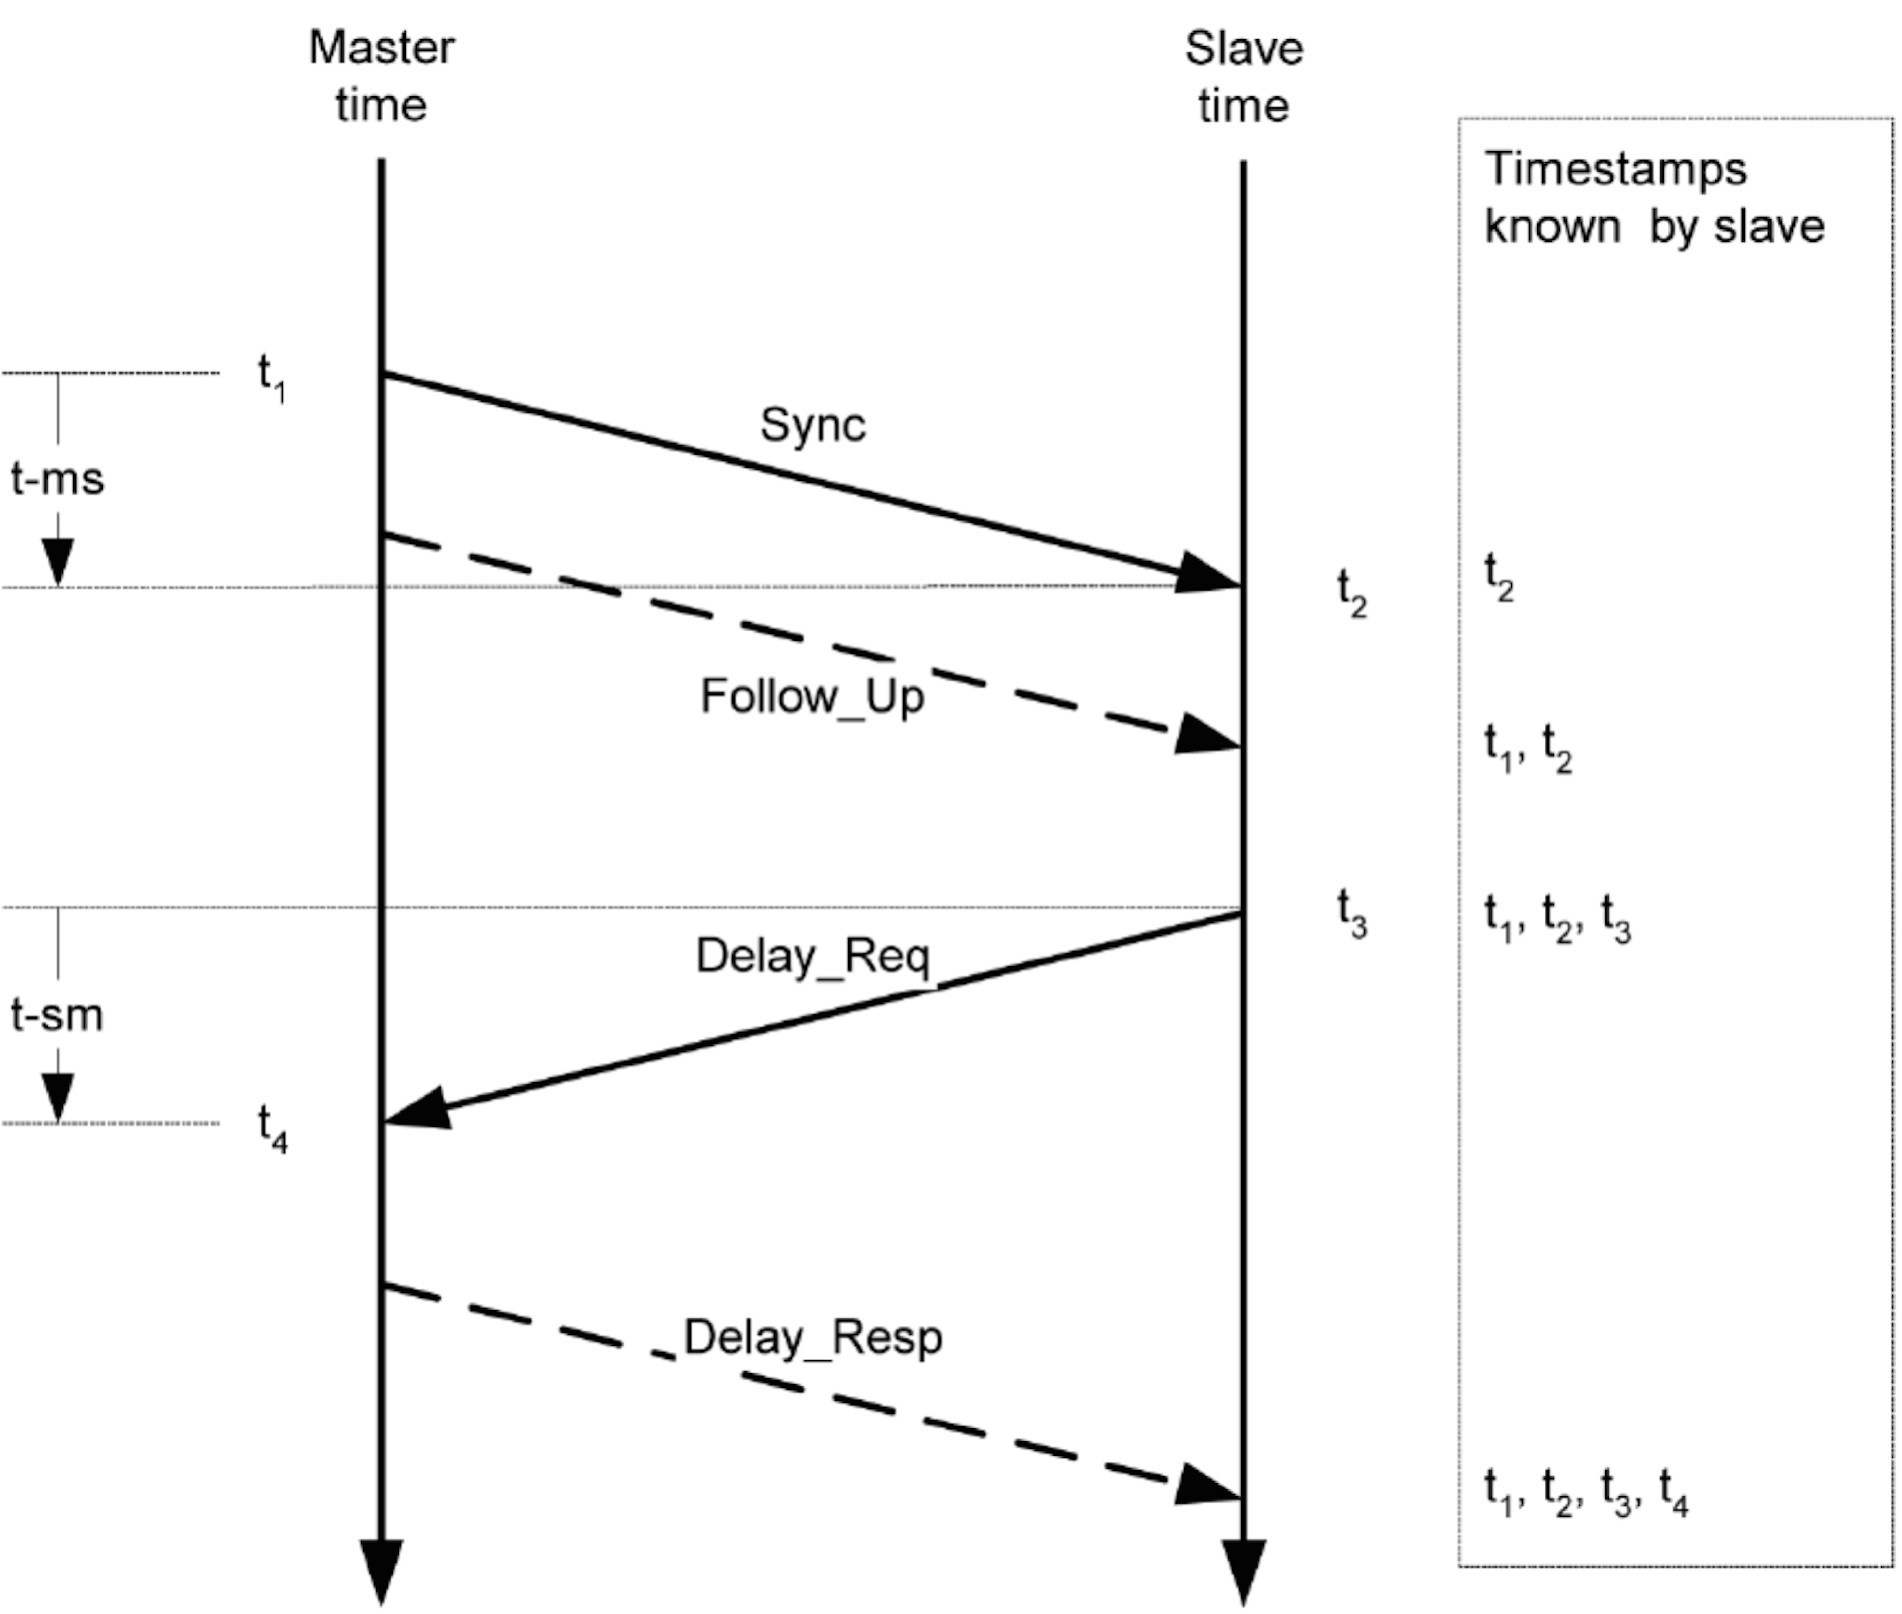
\includegraphics[width=10cm]{process_of_time_sync}
    \bicaption[fig:process_of_time_sync]{时钟同步算法流程图}{时钟同步算法流程图}{Fig}{Method of Time Sync}
  \end{minipage}     
\end{figure}

\subsection{时钟相位同步}
首先,主时钟会周期性对外发送Sync报文,当该报文离开主时钟时会记录时间戳为$t_{1}$。

然后,当从时钟接收到Sync报文时,标记接收时间为$t_{2}$。此时,从时钟即获得了Sync报文的发送与接收时间戳$t_{1}$和$t_{2}$。那么假设主从时间偏差为$T_{offset}$,主从时钟间网络传输时间为$T_{delay}$,则可以得到下面式子:
\begin{align}
	T_{offset} + T_{delay_1} = t_2 - t_1
\end{align}
另外,从时钟周期性向主时钟发送Delay\_Req报文,假设发送时间为$t_{3}$,当主时钟收到该报文时,会立即记录下Delay\_Req报文的接收时间$t_{4}$,并把该接收时间$t_{4}$存入Delay\_Resp报文中传递回该从时钟。那么此时,从时钟会得到$t_{3}$和$t_{4}$两个时间,可得到下面式子:
\begin{align}
	T_{delay_2} - T_{offset} = t_4 - t_3
\end{align}
此时,根据协议标准中,将往返传输延时视为对称,即:
\begin{align}
	T_{delay_1} = T_{delay_2} = T_{delay}
\end{align}
所以,结合上面几个式子可以得到如下结果:
\begin{align}
	T_{delay} = \frac{(t_2 - t_1) + (t_4 - t_3)}{2}
\end{align}
\begin{align}
	T_{offset} = \frac{(t_2 - t_1) - (t_4 - t_3)}{2}
\end{align}

通过上面的计算方法,可以得到主从时钟之间的相位偏差$T_{offset}$。然后,还需要计算主从时钟的时钟频率偏差才能实现完整的时钟同步。

\subsection{时钟频率同步}
在大多数情况下,主时钟设备会采用高稳时钟作为时间源,其频率一般非常稳定。但是,从时钟设备一般只会采用普通晶振源作为时钟源,其物理特性较差,容易受到外界环境和自身寿命等因素导致时钟漂移,这就导致了主从时钟由于频率差异而时时处于变化之中。因此,如果想要实现主从时钟的真正同步,就必须调节从时钟频率以使其保持与主时钟一致,从而缓解同步误差的根本来源。

为了计算时钟频率偏差,假设主时钟是按固定周期向从时钟发送Sync报文,那么,对主时钟而言,第(k-1)个Sync报文和第(k)个Sync报文之间的发送间隔\supercite{6}为:
\begin{align}
	\Delta T_{master} = T_{master(k)} - T_{master(k - 1)}
\end{align}
其中,$T_{master(k)}$表示第k个Sync报文的主时钟发送时间。

对于从时钟而言,两个Sync报文的时间间隔\supercite{6}为:
\begin{align}
	\Delta T_{slave} = T_{slave(k)} - T_{slave(k - 1)}
\end{align}
其中,$T_{slave(k)}$表示第k个Sync报文的在从时钟处的接收时间。由此得到主从时钟的频率偏差。
\begin{align}
	\Delta f = \frac{\Delta T_{master}}{\Delta T_{slave}}
\end{align}
因此,可以对从时钟的晶振设备进行调节,将其本地频率扩大$\Delta f$倍,即可实现主从时钟频率一致。通过不断对从时钟晶振源频率进行调节,可以减小主从时钟的计时速率偏差,从根本上减小了主从时钟偏差的来源。

为了能够采用上述方法来进行频率调节,在实际运行中需要确保主时钟周期性对外发送PTP报文,例如Sync报文,在这样的前提下,从时钟只需要累计一定周期内Sync报文的发送时间和接收时间,利用这些数据可以对主从时钟的频率差进行估计。

\section{同步精度的影响因素}
通过对时钟相位、频率同步原理的分析,可以知道整个同步系统会受到多种因素干扰,这些因素不仅会破坏报文传输过程,还会影响到主从时钟频率误差。因此,如果想要实现精确的时钟同步,不仅要利用同步算法把主从时钟偏差计算出来,还需要通过PTP报文的主从传输周期计算出从时钟的频率漂移补偿量。下面对同步过程中破坏相位、频率的因素进行分析。

\subsection{PTP报文传输周期}
在同步过程中,最基本的是$T_{offset}$值和$T_{delay}$值的计算,这将直接影响同步结果的准确性和稳定性,以及最初PTP网络建立的快速性。IEEE1588协议中报文包括事件报文和报文,相关的报文周期和超时事件如下。
\begin{itemize}[noitemsep,topsep=0pt,parsep=0pt,partopsep=0pt]
	\item Announce报文周期:AnnounceInterval默认值为2s,采用多播方式发送Announce报文。当从时钟接收到该报文,若端口为Slave状态,则会更新本地数据集。该报文主要用于最佳主时钟算法,报文内部包含描述主时钟所需的数据集,当时钟接收到该报文时,即会调用最佳主时钟算法,比较自身与外部时钟的品质,并根据结果来决定端口的主从状态\supercite{52}。所以,如果报文周期太长,那么系统建立主从状态则需要花费较多的时间,但如果周期太短,则造成网络拥挤和频繁主从状态刷新。
	\item Sync报文周期:SyncInterval参考值为0.5s-2s。每个Master端口会周期性对外发送Sync报文,该报文包含了主时钟发送时的时间戳。当从时钟接收到该报文,就会通过$T_{offset}$计算方法来计算出主从时间偏差,并以此来校正自身从而实现同步\supercite{52}。如果SyncInterval取值过大,则会使的从时钟偏离太大而失去同步效果;若该周期太小,则会严重加剧网络流量负载,从时钟处于不断的调整波动之中。
	\item Delay\_Req报文周期:MinDelayReqInterval参考值为1s-32s,默认1s。为了获得主从时钟间的路径传输延时,从时钟会周期性对主时钟发送Delay\_Req报文,当主时钟接收到该报文时,会立即保存接收时间戳,并通过回传Delay\_Resp报文把接收时间戳返回给从时钟,用于从时钟的$T_{delay}$值更新\supercite{52}如果周期过小,则会给主时钟增加过多的负载压力,加剧网络流量负载;若周期过大,则有可能导致上一次的$T_{delay}$与当前实际$T_{delay}$值出现严重偏差,从而导致$T_{offset}$值偏差较大,严重破坏同步精度。理想的周期应该在区间[0, $2^{MinDelayReqInterval+1}$]中均匀分布。
\end{itemize}

\subsection{链路延时不对称}
\label{sec:1588_problem_1}
如式子(2-4)、(2-5)所示,当计算主从时钟偏差$T_{offset}$时,需要先获取链路传输延时$T_{delay}$。在协议中该延时的计算方法是直接假设前后两次传输延时相等,从而通过取平均计算出$T_{offset}$。然而实际上,前后两次的传输路径往往并不对称,即式(2-3)并不成立,而导致往返的链路传输延时不一致的因素\supercite{55}如下。
\begin{itemize}[noitemsep,topsep=0pt,parsep=0pt,partopsep=0pt]
	\item 排队堵塞:当报文在传输中经过中间交换机或路由器时,由于网络负载的不可预知性,无法知道报文在中间交换机上的排队时间,当网络流量良好时,报文可以直接传递过去;而当网络负载较大,可能导致很长的报文排队时间。另外,即使报文可以不用排队,由于协议栈的存在,报文仍然需要经过解包和打包的过程,而这两个过程的消耗时间都与操作系统的调度和协议栈处理过程有关。因此,报文传递过程中穿越交换机时排队和堵塞时间的随机性会导致延时不对称\supercite{46}。
	\item 传输抖动:在网络系统中,所有信息的传递过程所消耗的时间会存在固有的抖动,这是无法避免的。
	\item 网络拓扑结构变化:当拓扑结构突然发生变化,报文传输的路径也就不同了,这必然导致往返链路时延完全不同。
	\item $T_{delay}$与当前真实延时不匹配:因为$T_{delay}$的计算依靠Delay\_Req报文周期,而$T_{offset}$的计算又是依靠Sync报文周期,两者一般并不匹配。所以会导致在计算$T_{offset}$所使用的$T_{delay}$是过去的值,与当前真实的$T_{delay}$值可能并不一致。
\end{itemize}

上述几种现象的存在,都会导致往返的两次延时不一致,所以说,在高同步精度的要求下,真实的传输延时绝对不能简单的假设相等。

\subsection{主从时钟源频率漂移}
由于主时钟在发送Sync报文时的偏差值$T_{offset1}$与从时钟最后接收Delay\_Resp报文时的偏差值$T_{offset2}$是不完全一致的,所以最终计算出来的$T_{offset}$并不完全等于真实的$T_{offset2}$。而且,在实际工业环境中,由于主时钟一般会采用更为稳定、精度较高的设备,而从时钟则一般精度较低,晶振源容易发生漂移现象,从而导致主从时钟之间的频率无法保持一致,这个因素会持续不断的使得从时钟偏离主时钟,因此,本文将对从时钟频率进行补偿,从而降低从时钟漂移现象对同步精度带来的破坏。

\subsection{时间戳的精确度}
\label{sec:1588_problem_2}
对于很多采用软件时间戳方式的设备,报文在协议栈中传递所带来的延时会导致物理层之上的时间戳往往不能真实反映报文的发送时间或接收时间,从而导致时间戳错误\supercite{53}。这也导致报文封装和解包过程产生偏差,直接破坏最终的时钟同步精度。本交换机项目中,采用的是支持硬件时间戳的设备,即设备能够直接在物理层为报文添加时间戳,从而保证了时间戳的精确度,因此,在本文将会忽略此因素。

\subsection{影响因素的优化方法}
提高时钟系统同步精度,也就意味着要提高主从时钟的相位与频率同步精度。因此,必须要针对上述影响同步精度的因素进行优化,降低这些因素对同步精度的影响。

对于PTP报文传输周期,需要结合PTP同步系统网络建立的快速性和网络负载压力来均衡考虑,可以在保证网络负载不至于太大的前提下,提高Announce报文的发送周期,以保证同步系统永远能和最佳主时钟进行同步。同样,Sync报文的发送有助于提高主从时钟的同步精度,更短的Sync报文周期意味着更频繁的主从同步过程,所以在工业现场中,如果发送时钟同步效果不太明显,而此时网络负载情况良好时,就可以选择加快Sync报文的发送以做更多次的时钟同步。对于Delay\_Req报文,主要是用来计算链路传输延时,如果链路处于较为稳定的状态,那么可以减少该报文的发送,而如果链路出现抖动或者链路结构发生了变化,那么就需要提高该报文发送速率,从而获得更为准确的链路传输时间。

链路延时的不对称性会直接影响到报文传输时间,从而导致主从时钟的相位偏差计算出错,进而破坏时钟相位同步效果。对于链路延时中的网络流量抖动,可以通过例如均值法、线性回归等方法,通过样本拟合来减小报文传输中的时延固有抖动;对于排队堵塞等,由于这种情况下链路延时会发生较大的变化,例如链路网络突然发生严重堵塞,那么PTP报文需要经过很长的时间才能在主从时钟之间传递,而对于从时钟而言它假设链路是对称的,从而产生严重误差,另一方面,排队堵塞一般只是暂时性的,即持续时间一般不会太久。因此可以对此类链路延时大幅抖动进行限制以免从时钟产生明显震荡。

从时钟源漂移现象会严重破坏时钟频率同步效果,一旦主从时钟频率无法同步,就意味着主从时钟会持续性产生时钟偏差,这是主从不同步的非常重要的来源。因此,必须去实时检测主从时钟的频率偏差,通过周期性发送PTP报文,来对主从时钟的本地频率进行检测。当然,在实际情况下不能保证主从时钟一定会周期性发送PTP报文,所以可以让主时钟会对外发送一个特有的频率Freq\_Sync同步报文,保证该报文的周期性发送,而从时钟也会专门检测该报文,并利用该报文来估算主从时钟本地频率来进行补偿。

\section{本章小结}
本章首先分析了IEEE1588时钟同步原理,即包括时钟同步中的相位与频率同步原理,阐述了时间同步的计算方法。另外,还针对相位与频率同步中的影响因素进行了细致的分析,包括PTP报文传输周期、链路延时不对称性和从时钟漂移等因素。这些因素都会不同程度的破坏时钟同步过程,降低时钟同步精度。最后,针对这些因素提出了相关的优化思路,利用这些优化方法可以提高相位与频率的同步效果。
